%**************************************************************************************
% License:
% CC BY-NC-SA 4.0 (http://creativecommons.org/licenses/by-nc-sa/4.0/)
%**************************************************************************************

\documentclass[handout]{beamer}

\mode<presentation> {

\usetheme{Madrid}

% Burnt orange
\definecolor{burntorange}{rgb}{0.8, 0.33, 0.0}
\colorlet{beamer@blendedblue}{burntorange}
% Pale yellow
\definecolor{paleyellow}{rgb}{1.0, 1.0, 0.953}
\setbeamercolor{background canvas}{bg=paleyellow}
% Secondary and tertiary palett
\setbeamercolor*{palette secondary}{use=structure,fg=white,bg=burntorange!80!black}
\setbeamercolor*{palette tertiary}{use=structure,fg=white,bg=burntorange!60!black}

% To remove the footer line in all slides uncomment this line
%\setbeamertemplate{footline}
% To replace the footer line in all slides with a simple slide count uncomment this line
%\setbeamertemplate{footline}[page number]

% To remove the navigation symbols from the bottom of all slides uncomment this line
%\setbeamertemplate{navigation symbols}{}
}

\usepackage{amsmath}
\usepackage{bm}
\usepackage{breqn}
\usepackage{fontawesome}
\usepackage{graphicx} % for figures
\usepackage{subcaption} % for subplots 
\usepackage[labelsep=space,tableposition=top]{caption}
\renewcommand{\figurename}{Fig.} 
\usepackage{cleveref}
\usepackage{caption,subcaption}% http://ctan.org/pkg/{caption,subcaption}
\usepackage{booktabs} % Allows the use of \toprule, \midrule and \bottomrule in tables
\usepackage{multirow}
\usepackage{xcolor}
\usepackage{empheq}
\usepackage[most]{tcolorbox}
\usepackage{listings}% http://ctan.org/pkg/listings
\lstset{basicstyle=\ttfamily,breaklines=true}
\usepackage{siunitx}
\usepackage{verbatim}

% To print 2 slides on a page
%\usepackage{handoutWithNotes}
%\pgfpagesuselayout{2 on 1}[border shrink=2mm]
%----------------------------------------------------------------------------------------
%	TITLE PAGE
%----------------------------------------------------------------------------------------
% The short title appears at the bottom of every slide, the full title is only on the title page
\title[CE 311K: Intro to Computer Methods]{CE 311K: Introduction to Computer Methods} 
\author{Krishna Kumar} % name
\institute[UT Austin] % institution 
{
University of Texas at Austin \\
\medskip
\href{mailto:krishnak@utexas.edu}{krishnak@utexas.edu} % email address
}
\date{} % Date, can be changed to a custom date

\begin{document}

\begin{frame}
\titlepage % title page as the first slide
\end{frame}



\begin{frame}
 % Table of contents slide, comment this block out to remove it
 \frametitle{Overview}
 % Throughout your presentation, if you choose to use \section{} and \subsection{} 
 % commands, these %will automatically be printed on this slide as an overview 
 \tableofcontents
 \textcolor{blue}{\faQuestionCircleO ~How are you feeling this morning?}
\end{frame}

\newif\ifshowtoc
\showtoctrue% toggles to show the toc

\AtBeginSection{%
	\ifshowtoc
	\begin{frame}
		\tableofcontents[currentsection, subsectionstyle=show/show/hide]
	\end{frame}
	\fi
}

%----------------------------------------------------------------------------------------
% slides
%----------------------------------------------------------------------------------------
%------------------------------------------------
\begin{frame}
	\frametitle{What is an algorithm?}
	\begin{figure}[ht]
		\centering
		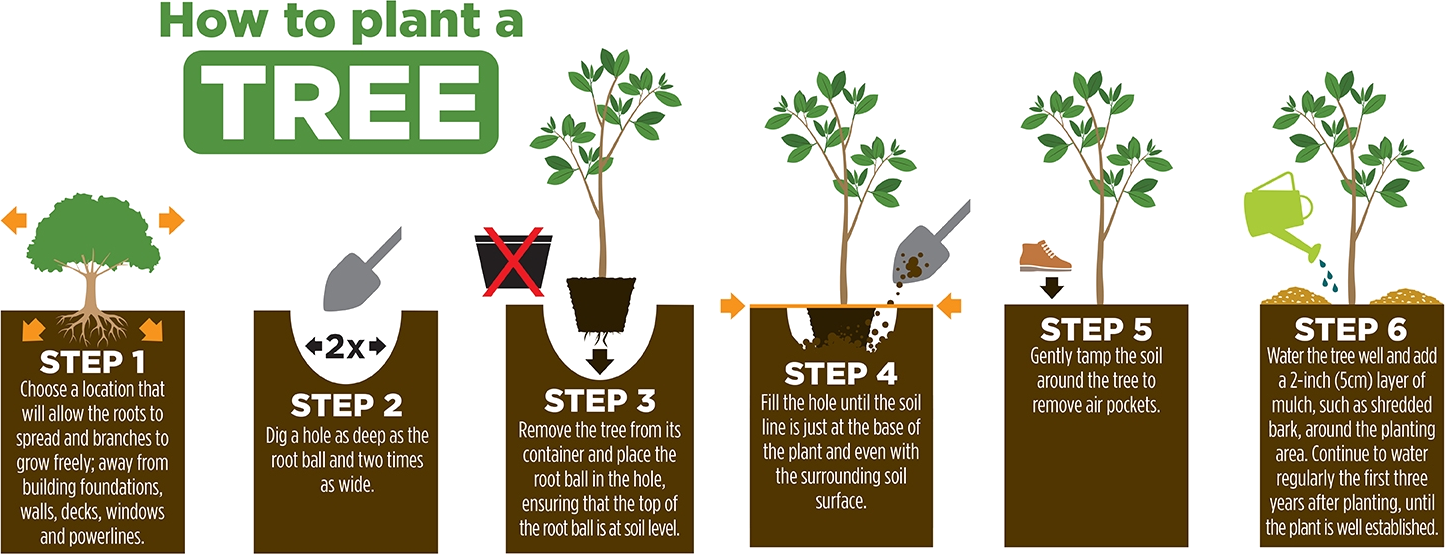
\includegraphics[width=0.92\textwidth]{figs/plant-tree.png}
	\end{figure}
	\textcolor{blue}{\faQuestionCircleO ~Could you identify examples of algorithms in real-world?}
\end{frame}
\note{An algorithm is a finite sequence of well-defined, computer-implementable instructions, typically to solve a class of problems or to perform a computation.}

%------------------------------------------------
\begin{frame}
	\frametitle{The Prophet and the Pioneer Computer Scientists}
	\begin{minipage}[t]{0.49\linewidth}
		\begin{figure}[ht]
			\centering
			\includegraphics[width=0.8\textwidth]{figs/ada-lovelace.jpg}
			\caption*{Ada Lovelace, circa 1838 (credit: Science Museum, California)}
		\end{figure}
	\end{minipage}%
	\hfill%
	\begin{minipage}[t]{0.49\linewidth}
		\begin{figure}[ht]
			\centering
			\includegraphics[width=0.92\textwidth]{figs/grace-hopper.jpg}
			\caption*{Grace Hopper (credit: unknown)}
		\end{figure}
	\end{minipage}
\end{frame}

\note{
	Lovelace speculated that the Engine `might act upon other things besides number... the Engine might compose elaborate and scientific pieces of music of any degree of complexity or extent'. The idea of a machine that could manipulate symbols in accordance with rules and that number could represent entities other than quantity mark the fundamental transition from calculation to computation.
	
	Hopper is the pioneer computer scientist, known for creating COBOL – the first computing language. There are over 220 billion lines of COBOL in existence, a figure which equates to around 80\% of the world's actively used code. There are estimated to be over a million COBOL programmers in the world today. Most impressive perhaps, is that 200 times as many COBOL transactions take place each day than Google searches, which is 5.6 billion queries/day.
}

%------------------------------------------------
\begin{frame}[fragile]
	\frametitle{On computable numbers}
	\begin{figure}[ht]
		\centering
		\includegraphics[width=\textwidth]{figs/turing-bombe.png}
		\caption*{Enigma has 150,738,274,937,250 possible states. (credit: Rutherford journal)}
	\end{figure}
	Decipher this text from an Engima machine:
	\begin{verbatim}
	KLDP AXKR MIMS VNUK M
	\end{verbatim}
\end{frame}

\note{
	Turing began to consider whether a method or process could be devised that could decide whether a given mathematical assertion was provable. Turing analyzed the methodical process, focusing on logical instructions, the action of the mind, and a machine that could be embodied as a physical form. Turing developed the proof that automatic computation cannot solve all mathematical problems. This concept became known as the Turing machine, which has become the foundation of the modern theory of computation and computability.
	
	KLDP AXKR MIMS VNUK M is Welcome to UT Austin
}

%------------------------------------------------
\begin{frame}
	\frametitle{To infinity and beyond...}
	\begin{figure}[ht]
		\centering
		\includegraphics[width=\textwidth]{figs/hamilton-bouman.png}
		\caption*{Margaret Hamilton next to a stack of the Apollo Guidance Computer source code (1969, credit: MIT Museum) and Katie Bouman who developed the algorithm for creating the first-ever image of black hole (2019, credits: PBS).}
	\end{figure}
	\textcolor{blue}{\faQuestionCircleO ~Could you guess the storage size requirements?}
\end{frame}

\note{
	Margaret Hamilton next to a stack of the Apollo Guidance Computer source code (1969, with 11,000 lines of code running on \textbf{72 kilobytes} of computer memory, credits: MIT Museum) and Katie Bouman who developed the algorithm for creating the first-ever image of black hole (2019, credits: PBS) and the HDD of \textbf{5 petabytes} of data. 
	
	If we assume a typical MP3 song as 4MB, we can fit ~56 Apollo guidance code in a song, while the 5 PetaBytes of data can hold 250 million songs (there are roughly ~97 million songs in the world.)
}

%------------------------------------------------
\begin{frame}
	\frametitle{To infinity and beyond...}
	\begin{figure}[ht]
		\centering
		\includegraphics[width=0.55\textwidth]{figs/blackhole.png}
	\end{figure}
\end{frame}

\note{
	Scientists have obtained the first image of a black hole, using Event Horizon Telescope observations of the center of the galaxy M87. The image shows a bright ring formed as light bends in the intense gravity around a black hole that is 6.5 billion times more massive than the Sun. The task of observing this super massive black hole is extremely hard, the size ratio is same as observing an orange on the surface of moon from the Earth.
}

\section{Simulations}
%------------------------------------------------
\begin{frame}
\frametitle{Disney's Frozen: Modeling snow}
\begin{figure}[ht]
	\centering
	\includegraphics[width=\textwidth]{figs/anna-before-snow.png}
\end{figure}
\end{frame}

%------------------------------------------------
\begin{frame}
	\frametitle{\faQuestionCircleO  How to bury Anna under the snow?}
	\begin{figure}[ht]
		\centering
		\includegraphics[width=\textwidth]{figs/anna-snow.png}
		
	\end{figure}
\end{frame}

%------------------------------------------------
\begin{frame}
	\frametitle{Modeling the real world: Spherical Cow}
	\begin{figure}[ht]
		\centering
		\includegraphics[width=0.65\textwidth]{figs/spherical-cow.png}
	\end{figure}
\end{frame}

%------------------------------------------------
\begin{frame}
	\frametitle{Modeling snow}
	\begin{figure}[ht]
		\centering
		\includegraphics[width=\textwidth]{figs/snow-model.png}
	\end{figure}
\end{frame}

%------------------------------------------------
\begin{frame}
	\frametitle{How to animate like Disney: Effect of snow quantity}
	\begin{figure}[ht]
		\centering
		\includegraphics[width=\textwidth]{figs/anna-quantity-snow.png}
	\end{figure}
\end{frame}

%------------------------------------------------
\begin{frame}
	\frametitle{What type of snow?}
	\begin{figure}[ht]
		\centering
		\includegraphics[width=\textwidth]{figs/snow-types.png}
	\end{figure}
\end{frame}

%------------------------------------------------
\begin{frame}
	\frametitle{Snow properties}
	\begin{figure}[ht]
		\centering
		\includegraphics[width=\textwidth]{figs/snow.png}
	\end{figure}
\end{frame}

%------------------------------------------------
\begin{frame}
	\frametitle{Snow material parameters}
	\begin{figure}[ht]
		\centering
		\includegraphics[width=0.9\textwidth]{figs/snow-parameters.png}
	\end{figure}
\end{frame}


%------------------------------------------------
\begin{frame}
	\frametitle{How to model snow?}
	\begin{minipage}[t]{0.59\linewidth}
	\mode<beamer>{
		\begin{itemize}
			\item Representation of snow: Each snow flake is modeled as a particle
			\item Physics: our model or parameters of how the snow behaves
			\item Solver: How the snow would move and interact with the objects in the scene.
			\item Algorithm: A sequence of logical steps required to perform a specific task.
			\item Implementation and verification of our snow model.
		\end{itemize}
		\faLightbulbO~\textcolor{green}{This is a \textbf{simulation}.}
	}
	\mode<handout>{
		\vspace{5cm}
	}
	\end{minipage}%
	\hfill%
	\begin{minipage}[t]{0.39\linewidth}
		\begin{figure}[ht]
			\centering
			\includegraphics[width=0.7\textwidth]{figs/anna-in-snow.png}
		\end{figure}
	\end{minipage}
\end{frame}

\note{
	 A simulation is an approximate imitation of the operation of a process or system. The first step is to create model, which represents the system's key characteristics, such as its behavior, functions and abstract or physical properties. The model represents the system itself, whereas the simulation represents its operation over time.	
	 
	 There are several numerical techniques that can be used to solve a mathematical problem. They differ in accuracy, length of calulations, and difficulty in programming.
	 
	 Since numerical solutions are an approximation and  the computer program that executes the numerical method might have errors (or bugs), a numerical solution needs to be examined closely.
}

%------------------------------------------------
\section{Aspects of languages}
%------------------------------------------------
\begin{frame}
	\frametitle{\faCommentsO ~What does a computer do?}
	\mode<beamer>{
		\begin{itemize}
			\item Fundamentally:
			\begin{itemize}
				\item performs \textit{calculations} - a billion calculations per second.
				\item Remembers results 100s of gigabytes of storage.
			\end{itemize}
		\item Computers only know and do what you tell them!
		\item \textbf{Fixed program} computer (calculator)
		\item \textbf{Stored program} computer - machine stores and executes instructions
	\end{itemize}
	}
	\mode<handout>{
		\vspace{3cm}
	}
	\begin{figure}[ht]
		\centering
		\includegraphics[width=0.6\textwidth]{figs/bluegene.png}
		\caption*{IBM Bluegene/P supercomputer (credit: unknown)}
	\end{figure}
\end{frame}
\note{A single rack of IBM Bluegene/P in 2007 could do 5Terra flops as fast as the current iPhones X.

UT Austin's Frontera can do 38 PetaFlops. In contrast a human brain can do 1,000 petaflops or 10 quadrillion operations per second (i.e., 1 exaflop or a billion - billion calculations).
}

%------------------------------------------------
\begin{frame}[fragile]
	\frametitle{Companies using python}
	\begin{figure}[ht]
		\centering
		\includegraphics[width=\textwidth]{figs/python-companies.png}
	\end{figure}
\end{frame}

%------------------------------------------------
\begin{frame}
	\frametitle{\faCommentO ~What are the primary aspects of a language?}
	\mode<beamer>{
		\begin{itemize}
			\item Primitive constructs (objects and operators)
			\item Syntax
			\item Static semantics
		\end{itemize}
	}
	\mode<handout>{
		\vspace{5cm}
	}
\end{frame}

%------------------------------------------------
\begin{frame}
	\frametitle{Aspects of languages: Primitive constructs}
	\mode<beamer>{
		\begin{itemize}
			%\item Turing showed that you can compute anything using \textbf{6 			primitives}.
			\item \textit{English}: words and punctuations
			\item \textit{Programming languages}: numbers, strings, simple operators
			\item Anything computable in one language is computable in
			any other programming language.
		\end{itemize}
	}
	\mode<handout>{
		\vspace{3cm}
	}
	\begin{minipage}[t]{0.59\linewidth}	
		\begin{figure}[ht]
			\centering
			\includegraphics[width=\textwidth]{figs/english-word-cloud.png}
			\caption*{English word cloud (credit: Michael Twardos)}
		\end{figure}
	\end{minipage}%
	\hfill%
	\begin{minipage}[t]{0.39\linewidth}
		\begin{figure}[ht]
			\centering
			\includegraphics[width=0.7\textwidth]{figs/python-word-cloud.png}
			\caption*{Python word cloud \\ (credit: unknown)}
		\end{figure}
	\end{minipage}%
\end{frame}

\note{In fact, Alan Turing, who was a really great computer scientist, he showed that you can compute anything using the six primitives. And the six primitives are move left, move right, read, write, scan, and do nothing. Using those six instructions and the piece of tape, he showed that you can compute anything. And using those six instructions, programming languages came about that created a more convenient set of primitives. You don't have to program in only these six commands.}

%------------------------------------------------
\begin{frame}
	\frametitle{Python program}
	\begin{itemize}
		\item We'll be using Python 3.x 
		\item a program is a sequence of definitions and commands
		\mode<beamer>{
			\begin{itemize}
				\item \textbf{definitions} \textit{evaluated}
				\item \textbf{commands (statements)} instructs Python interpreter (program) to \textit{execute} something
			\end{itemize}
		}
		\mode<handout>{
			\vspace{2cm}
		}
		\item programs manipulate \textbf{data objects}
		\item objects are
		\mode<beamer>{
			\begin{itemize}
				\item \textbf{scalar} (cannot be subdivided)
				\item \textit{non-scalar} (have internal structure that can be accessed)
			\end{itemize}
			objects have a \textbf{type} that defines the kinds of things
			programs can do to them. For example a list of items.
		}
		\mode<handout>{
			\vspace{2cm}
		}
	\end{itemize}
\end{frame}

%------------------------------------------------
\begin{frame}[fragile]
	\frametitle{Scalar objects}
	\mode<beamer>{
		\begin{itemize}
			\item \texttt{int}: represent integers, e.g., \texttt{5}
			\item \texttt{float}: represent real numbers, e.g., \texttt{3.27}
			\item \texttt{bool}: represent Boolean values \texttt{True} and \texttt{False}
			\item \texttt{str}: A sequence of characters (can contain unicode characters). 
			e.g., \texttt{``Hi!'' ``$\theta$''} 
			\item \texttt{NoneType}:  special and has one value, \texttt{None}
			\item can use \texttt{type()} to see the type of an object
		\end{itemize}
	}
	\mode<handout>{
		\vspace{4cm}
	}
	\begin{lstlisting}[language=Python]
	In [1]: type(5)
	Out[1]: int
	In [2]: type(3.0)
	Out[2]: float
	\end{lstlisting}
\end{frame}

%------------------------------------------------
\begin{frame}[fragile]
	\frametitle{Printing to console}
	To show the output from code to a user \verb|print| command:
	\begin{figure}[ht]
		\centering
		\includegraphics[width=0.6\textwidth]{figs/shell-print.png}
	\end{figure}
\end{frame}

%------------------------------------------------
\begin{frame}
	\frametitle{Aspects of languages: Syntax and Static semantics}
	\textit{\textbf{Syntax}}
	\mode<beamer>{
		\begin{itemize}
			\item \textit{English} 
			\begin{itemize}
				\item ``\textit{boy dog cat}'': \mode<beamer>{syntactically invalid}
				\item ``\textit{boy hugs cat}'': \mode<beamer>{syntactically valid}
			\end{itemize}
			\item \textit{Python} 
			\begin{itemize}
				\item \texttt{5 "Hi"}: \mode<beamer>{syntactically invalid}
				\item \texttt{3.2 * 7}: \mode<beamer>{syntactically valid}
			\end{itemize}
		\end{itemize}
	}
	\mode<handout>{
		\vspace{3cm}
	}
	\textit{\textbf{Static semantics}} is when syntactically valid strings have meaning:
	\mode<beamer>{	
		\begin{itemize}
			\item English: ``\textit{I are hungry}'': syntactically valid, 	but static semantic error
			\item Python: \texttt{5 + "Hi"}: syntactically valid, but static semantic error
		\end{itemize}
	}
	\mode<handout>{
		\vspace{3cm}
	}
\end{frame}

%------------------------------------------------
\begin{frame}
	\frametitle{Aspects of languages: Semantics}
	Semantics is the meaning associated with a syntactically correct string of symbols with no static semantic errors:
	\begin{itemize}
		\item \textit{English}: can have many meanings ``Flying planes can be dangerous''.
		\item \textit{programming languages}: have only one meaning but may not be what programmer intended		
	\end{itemize}
\end{frame}

%------------------------------------------------
\begin{frame}[fragile]
	\frametitle{Expressions and operations}
	\mode<beamer>{	
		\begin{itemize}	
			\item \textbf{combine objects and operators} to form \textit{expressions}
			\item an expression has a value, which has a type
			\item syntax for a simple expression:
			$<object> <operator> <object>$
		\end{itemize}
	}
	\mode<handout>{
		\vspace{3cm}
	}
	\begin{itemize}	
		\item Operations on `ints' and `floats':
		\item \verb|i + j|: \textit{sum} (int or float)
		\item \verb|i - j|: \textit{difference} (int or float)	
		\item \verb|i * j|: \textit{product} (int or float)
		\item \verb|i / j|: \textit{division} (float)
		\item \verb|i % j|: \textit{remainder} of \verb|i| divided by \verb|j|
		\item \verb|i ** j|: \verb|i| to the \textit{power} of \verb|j|
	\end{itemize}
\end{frame}


%------------------------------------------------
\begin{frame}[fragile]
	\frametitle{Operator precedence}
	\begin{table}[!h]
		\begin{tabular}{ll}
			\toprule
			\verb|()| & Parantheses (grouping)  \\
			\verb|**| & Exponential \\
			\verb|+x, -x| & Positive, negative \\
			\verb|*, /, %| & Multiplication, division, remainder \\
			\verb|+, -| & Addition, subtraction \\
			\bottomrule
		\end{tabular}
	\end{table}
	If at equal level terms are evaluated from left to right.
\end{frame}
%------------------------------------------------
\begin{frame}
	\frametitle{Where things can go wrong}
	\mode<beamer>{
	\begin{itemize}
		\item \textbf{syntactic errors}: - common and easily caught
		\item \textbf{static semantic errors}:
		\begin{itemize}
			\item some languages check for these before running program
			\item can cause unpredictable behavior
		\end{itemize}
		\item no semantic errors \textbf{but different meaning than what
		programmer intended}
		\begin{itemize}
			\item program crashes, stops running
			\item program runs forever
			\item program gives an answer but different than expected		
		\end{itemize}
	\end{itemize}
	}
	\mode<handout>{
		\vspace{6cm}
	}
\end{frame}

%------------------------------------------------
\section{Python variables and bindings}
%------------------------------------------------
\begin{frame}[fragile]
	\frametitle{Binding variables and values}
	Equal sign is an \textbf{assignment} of a value to a variable name.
	\begin{lstlisting}[language=Python]
	pi = 3.14159
	pi_approx = 22/7
	\end{lstlisting}
	\mode<beamer>{
	\begin{itemize}
		\item value stored in computer memory
		\item an assignment binds name to value
		\item retrieve value associated with name or variable by invoking the name, by typing $pi$
		\item Why give names to values of expressions?
		\begin{itemize}
			\item to reuse names instead of values
			\item easier to change code later
		\end{itemize}
		\item Programming vs math: in programming, you do not ``\textit{solve for x}''. An assignment expression on the right, evaluated to a value. A variable name defined on the left stores the value(s).
	\end{itemize}
	}
	\mode<handout>{
		\vspace{5cm}
	}
\end{frame}

\note{
	\texttt{pi} is the variable 
	
	\texttt{3.14159} is the value
}

%------------------------------------------------
\begin{frame}[fragile]
	\frametitle{Changing bindings}
	\begin{itemize}
		\item can \textit{re-bind} variable names using new assignment
		statements
		\item previous value may still stored in memory but lost the
		handle for it
		\item value for area does not change until you tell the computer to do the calculation again
		\begin{lstlisting}[language=Python]
		pi = 3
		radius = 11
		area = 363
		radius = 14
		\end{lstlisting}
	\end{itemize}
	\mode<beamer>{
	\begin{minipage}[t]{0.49\linewidth}
	\begin{figure}[ht]
		\centering
		\includegraphics[width=0.62\textwidth]{figs/variable-binding.png}
	\end{figure}
	\end{minipage}%
	\hfill%
	\begin{minipage}[t]{0.49\linewidth}
		\begin{figure}[ht]
			\centering
			\includegraphics[width=0.62\textwidth]{figs/variable-binding-after.png}
		\end{figure}
	\end{minipage}
	}
	\mode<handout>{
		\vspace{3cm}
	}
\end{frame}

%------------------------------------------------
\begin{frame}[fragile]
	\frametitle{Engineering approximations}
	\begin{figure}[ht]
		\centering
		\includegraphics[width=0.62\textwidth]{figs/pi-e.png}
	\end{figure}
\end{frame}

%------------------------------------------------
\begin{frame}[fragile]
	\frametitle{Naming matters}
	\textcolor{blue}{\faQuestionCircleO ~What's wrong with the following code segment?}
	\begin{minipage}[t]{0.49\linewidth}
	\begin{lstlisting}[language=Python]
a = 3.14159
b = 11.2
c = a*(b**2)
print(c)
\end{lstlisting}
	\end{minipage}%
	\hfill%
	\begin{minipage}[t]{0.49\linewidth}
	\begin{lstlisting}[language=Python]
pi = 3.14159
diameter = 11.2
area = pi*(diameter**2)
print(area)
\end{lstlisting}
	\end{minipage}
\end{frame}
\note{As far as Python is concerned, they are not different. When executed, they will do the same thing. To a human reader, however, they are quite different. When we read the fragment on the left, there is no \textit{a priori} reason to suspect that anything is amiss. However, a quick glance at the code on the right sould prompt us to be suspicious that something is wrong. Either the variable should have been named \texttt{radius} rather than \texttt{diameter} or \texttt{diameter} should have been divided by \texttt{2.0} in the area calculation.}

\end{document}